\documentclass{book}
\usepackage{comment}
\usepackage{xcolor}
\usepackage{enumerate}
\usepackage{array}
\usepackage{amssymb}
\usepackage{amsmath}% http://ctan.org/pkg/amsmath
\usepackage{pgfplots}
\usepgfplotslibrary{fillbetween,decorations.softclip}
\pgfplotsset{compat = newest}
\usepackage[utf8]{inputenc}

 \newtheorem{theorem}{Theorem}[section]
\newtheorem{corollary}{Corollary}[theorem]
\newtheorem{lemma}[theorem]{Lemma}
 \newtheorem{definition}{Definition}[section]
 \newtheorem{example}{Example}[section]
 \newtheorem{remark}{Remark}[section]

\usepackage{geometry}
\usepackage{tcolorbox}
\usepackage{mathtools}

\DeclarePairedDelimiter\abs{\lvert}{\rvert}%
\usepackage[utf8]{inputenc}
\usepackage[colorlinks=true]{hyperref}


\definecolor{mygray}{gray}{0.8}
\definecolor{mygreen}{RGB}{200,255,200}
\definecolor{myred}{RGB}{255,210,210}
\definecolor{myblue}{RGB}{220,220,255}

\geometry{
 a4paper,
 left=5mm, 
 top=5mm
 }

\begin{comment}
      
\end{comment} 
\begin{comment}
      The 4 new commands listed below are for notation of sets for real, natural ,integer and complex numbers respectively
\end{comment} 

\hypersetup{
 urlcolor=blue,
 linkcolor= black,
}

\newcommand{\R}{\mathbb{R}}
\newcommand{\N}{\mathbb{N}}
\newcommand{\Z}{\mathbb{Z}}
\newcommand{\C}{\mathbb{C}}
\newcommand{\Q}{\mathbb{Q}}


\renewcommand*\contentsname{Index of Chapters}







\begin{document}
\begin{titlepage}
\centering
\vspace{5cm}
{\LARGE\bfseries Calculus and its Applications}

\vspace{1cm}

{\Large Taught by Professor Demetrios Papageorgiou}

\vspace{2cm}

{\Large Autumn 2019}

\vspace{2cm}

{\large Rahul Gupta , Javier Chico Vazquez , Francesco Piatti}

\vspace{5cm}

{\large THIS DOCUMENT IS MEANT TO BE VIEWED EXCLUSIVELY BY STUDENTS OF IMPERIAL COLLEGE LONDON STUDYING EITHER MATHS OR JMC!}

\end{titlepage}


\newpage
\tableofcontents{}
\newpage


\chapter{Preface}


Mathematics Year 1, Calculus and Applications\\~\\Assessment Information\\~\\
Calculus and Applications is a year-long course consisting of two parts, I and II, offered
in the Autumn and Spring terms, respectively.  You get one mark for both parts.  In what
follows details of the course assessment are given for the
whole course
(i.e.  a total mark of 100 \%) for (i) Mathematics students who take both parts I and II, and (ii) JMC students
who only take part I.\\~\\
Mathematics students parts I and II\\
Part I, Mid-term exam:\\
5\%\\
Part I, Portfolio marks:\\
5\%\\
Part I, January Test:\\
10\%\\
Part II, Mid-term exam:\\
5\%\\
Part II, Portfolio marks:\\
5\%\\
Summer Exam (Parts I and II, 3 hours):    70\%\\~\\
Joint Mathematics and Computing students part I only\\
Part I, Mid-term exam:\\
10\%\\
Part I, Portfolio marks:\\
10\%\\
Part I, January Test:\\
10\%\\
Summer Exam (Parts I only, 1.5 hours):    70\%\\
Brief overview of the syllabus - Derivatives , Theorems - (including but not limited to Intermediate Value Theorem , Mean Value Theorem) , Integration , Series , Taylor's Theorem , Power Series  Fourier Series and Fourier transforms

\chapter{Derivatives}
\section{Definition}

\begin{tcolorbox}[width=\textwidth,colback={mygray},title={\begin{definition}Derivative of a continuous function\end{definition}},colbacktitle=mygreen,coltitle=black]    

For any function , $f: X \to Y , y = f(x)$\\
We define $$f'(x)  =  \displaystyle\frac{df}{dx} = \lim_{h \to 0}\displaystyle\frac{f(x+h)-f(x)}{h}$$
\end{tcolorbox}

Make sure to consider the limits from both the left hand and the right hand side.\\

The limit can also be defined as $$f'(x)  \approx  \lim_{h \to 0}\displaystyle\frac{f(x+h)-f(x-h)}{2h}$$

\begin{tcolorbox}[width=\textwidth,colback={mygray},title={Example},colbacktitle=myred,coltitle=black]    

$f(x) = x^2$\\
$f'(x)  = Lim_{h \to 0}\displaystyle\frac{(x+h)^2-x^2}{h}$\\
       $f'(x)= Lim_{h \to 0}\displaystyle\frac{(2x+h)(h)}{h}$\\
       $f'(x)  = 2x$\\
\end{tcolorbox}

\begin{tcolorbox}[width=\textwidth,colback={mygray},title={\begin{example}Derivative of the absolute value\end{example}},colbacktitle=myred,coltitle=black]    

 \begin{equation}
  f(x) = \abs{x}=\left\{
    \begin{array}{@{} l c @{}}
      x & \text{$x \geq 0 $ } \\
      -x & \text{$ x < 0 $}
    \end{array}\right.
  \label{}
\end{equation}\\

  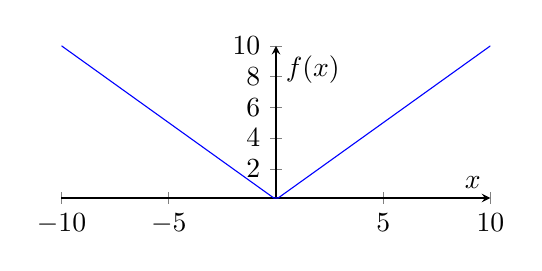
\begin{tikzpicture}
\begin{axis}[
     width=200,
    height=100,
    axis lines = center,
    xlabel = $x$,
    ylabel = {$f(x)$},
]
%Below the red parabola is defined
\addplot [
    domain=-10:10, 
    samples=100, 
    color=blue,
]
{abs(x)};

\end{axis}
\end{tikzpicture}\\
\underline{RHL}:\\ $f'(x)  = Lim_{h \to 0 , h > 0 }\displaystyle\frac{f(0+h)-f(0)}{h}$\\
       $f'(x)= Lim_{h \to 0 , h > 0}\displaystyle\frac{h-0}{h} = 1$\\~\\~\\
\underline{LHL}:\\ $f'(x)  = Lim_{h \to 0 , h < 0 }\displaystyle\frac{f(0+h)-f(0)}{h}$\\
       $f'(x)= Lim_{h \to 0 , h < 0}\displaystyle\frac{(-h-0)}{h} = -1$\\~\\~\\
       
       Right and left hand derivative exist.\\But $f'(0)$ doesn't .

\end{tcolorbox}

\begin{tcolorbox}[width=\textwidth,colback={mygray},title={Example},colbacktitle=myred,coltitle=black]    

 \begin{equation}
  f(x) =\left\{
    \begin{array}{@{} l c @{}}
      x & \text{$0  < x \leq 1 $ } \\
      x-1 & \text{$ 1 < x \leq 2 $}
    \end{array}\right.
  \label{}
\end{equation}\\

  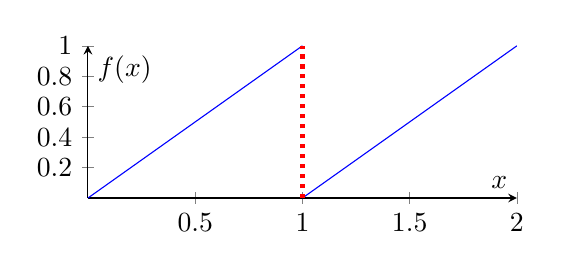
\begin{tikzpicture}
\begin{axis}[
     width=200,
    height=100,
    axis lines = center,
    xlabel = $x$,
    ylabel = {$f(x)$},
]
%Below the red parabola is defined
\addplot [
    domain=0:1, 
    samples=100, 
    color=blue,
]
{x};
\addplot [
    domain=1:2, 
    samples=100, 
    color=blue,
]
{x-1};
\draw [ultra thick, dotted, draw=red] 
        (axis cs: 1,0) -- (axis cs: 1,1)
        node[pos=0.5, above] {};

\end{axis}
\end{tikzpicture}\\

\underline{RHL}:\\ $f'(x)  = Lim_{h \to 0 , h > 0 }\displaystyle\frac{f(1+h)-f(1)}{h}$\\
       $f'(x)= Lim_{h \to 0 , h > 0}\displaystyle\frac{(1+h-1)-1}{h} =Lim_{h \to 0 , h > 0} 1 +\frac{-1}{h}$ which is undefined\\~\\~\\
\underline{LHL}:\\ $f'(x)  = Lim_{h \to 0 , h < 0 }\displaystyle\frac{f(1+h)-f(1)}{h}$\\
       $f'(x)= Lim_{h \to 0 , h < 0}\displaystyle\frac{(1+h)-1}{h} = 1$\\~\\~\\
       
       Right and left hand derivative exist.\\But $f'(1)$ doesn't .

\end{tcolorbox}


\section{Polynomials}
\begin{tcolorbox}[width=\textwidth,colback={mygray},title={\begin{theorem} Let $n \geq 1$ be any integer. Then  $f(x) = x^n$ , then $f'(x) = n x^{n-1}$ \end{theorem}},colbacktitle=myblue,coltitle=black] 
\underline{Proof:}\\
$=\lim_{h \to 0 }\displaystyle\frac{(x+h)^n- x^n}{h} =$\\
$=\lim_{h \to 0 }\displaystyle\frac{x^n + nhx^{n-1} + h^2 g(x,h) - x^n}{h}$ (using the binomial theorem)\\
$=\lim_{h \to 0 } nx^{n-1} + h g(x,h) =$ \\
$= \displaystyle n x^{n-1}$


\end{tcolorbox}

\section{General rules for differentiation}
We will show the derivative is a linear operator and how to differentiate products and quotients of functions.

\begin{theorem}Basic rules of differentiation


\begin{enumerate}
    \item [1)] $\forall k  \in \R $ ,$ f'(k) = 0 $\\~\\
    \underline{Proof:}\\
    $f' ( x ) = \lim_{h \to 0}\displaystyle\frac{f ( x + h ) - f ( x )}{h} = \lim_{h \to 0} \displaystyle\frac{k - k}{h} = \lim_{h \to 0} 0 = 0$\\~\\
    \item [2)] $\forall k  \in \R $ ,$ (kf(x))' = kf'(x) $\\~\\
    \underline{Proof:}\\
    $( k f ( x ) )' = \lim_{h \to 0} \displaystyle\frac{k f ( x + h ) - k f ( x )}{h} = k \lim_{h \to 0} \displaystyle\frac{f ( x + h ) - f ( x )}{h} = k f' ( x )$
    \item [3)] $  (f(x)+g(x))' = f'(x) \pm g'(x)  $\\~\\
    \underline{Proof:}\\\underline{For +:}\\
    $(f(x)+g(x))' = \lim_{h \to 0}\displaystyle\frac{f ( x + h ) + g(x+h) - (f ( x ) + g(x))}{h} \\= \lim_{h \to 0} \displaystyle\frac{f(x+h) - f(x)}{h}+ \lim_{h \to 0} \displaystyle\frac{g(x+h) - g(x)}{h} = f'(x) + g'(x)$\\~\\
    \\\underline{For -:}\\
    $(f(x)-g(x))' = \lim_{h \to 0}\displaystyle\frac{f ( x + h ) - g(x+h) - (f ( x ) - g(x))}{h} \\= \lim_{h \to 0} \displaystyle\frac{f(x+h) - f(x)}{h}- \lim_{h \to 0} \displaystyle\frac{g(x+h) - g(x)}{h} = f'(x) - g'(x)$\\~\\
    \item [4)] $  (f(x)\times g(x))' = f'(x)g(x) + f(x)g'(x)  $\\~\\
    \underline{Proof:}\\
    $((f(x)\times g(x))' = \lim_{h \to 0}\displaystyle\frac{f ( x + h )g(x+h) - f ( x )  g(x)}{h} \\= \lim_{h \to 0}\displaystyle\frac{f ( x + h )g(x+h) -f(x+h)g(x) + f(x+h)g(x)- f ( x )  g(x)}{h} \\= \lim_{h \to 0} \displaystyle\frac{f(x+h)(g(x+h) - g(x))}{h}+ \lim_{h \to 0} \displaystyle\frac{g(x)(f(x+h) - f(x))}{h} = \\= (\lim_{h \to 0} f(x+h))\lim_{h \to 0} \displaystyle\frac{(g(x+h) - g(x))}{h}+ (\lim_{h \to 0} g(x+h))\lim_{h \to 0} \displaystyle\frac{(f(x+h) - f(x))}{h}\\ = f(x)g'(x) + g(x)f'(x)$\\~\\
    \item [5)] $  \left({\displaystyle\frac{f(x)}{g(x)}}\right)' = \displaystyle\frac{f'(x)g(x) - g'(x)f(x)}{g(x)^2}  $\\~\\
    \underline{Proof:}\\
    $\left({\displaystyle\frac{f(x)}{g(x)}}\right)' \\~\\ = \lim_{h \to 0} \displaystyle\frac{\frac{f(x+h)}{g(x+h)} - \frac{f(x)}{g(x)} }{h} \\~\\ = \lim_{h \to 0} \displaystyle \frac{1}{h}\frac{f(x+h)g(x) - f(x)g(x)+f(x)g(x) - f(x)g(x+h)}{g(x+h)g(x)} \\~\\= \lim_{h \to 0} \displaystyle \frac{1}{g(x+h)g(x)}\left(\frac{f(x+h)g(x) - f(x)g(x)+f(x)g(x) - f(x)g(x+h)}{h}\right) \\~\\ = \lim_{h \to 0} \displaystyle \frac{1}{g(x+h)g(x)}\left(\left(\frac{f(x+h)g(x) - f(x)g(x)}{h}\right)+\left(\frac{f(x)g(x) - f(x)g(x+h)}{h}\right)\right) \\~\\ $Using the definition of a derivative and factoring out g(x) and f(x) ,$ \\~\\ =  \lim_{h \to 0} \displaystyle \frac{f'(x)g(x) - g'(x)f(x)}{g(x) \times g(x)} = \displaystyle\frac{f'(x)g(x) - g'(x)f(x)}{g(x)^2}$  \\~\\
    \\~\\
\end{enumerate}
\end{theorem}
\section{Chain Rule}

\begin{tcolorbox}[width=\textwidth,colback={mygray},title={\begin{theorem}If $h(x)=f(g(x))$. Then $h$ is differentiable at $x$ and:
$$h'(x)=f'(g(x))g'(x)$$ \end{theorem}},colbacktitle=myblue,coltitle=black]    
\underline{Proof:}\\ We will use the old but trustworthy trick of multiplying times one: $$h'(x)=\lim_{h\rightarrow0}\frac{f(g(x+h))-f(g(x))}{h}\frac{g(x+h)-g(x)}{g(x+h)-g(x)}$$
Let $k=g(x+h)-g(x)$, $u=g(x)$:
$$\lim_{h\rightarrow0}\frac{f(u+k)-f(u)}{k}\frac{g(x+h)-g(x)}{h}=f'(u)g'(x) = f'(g(x))g'(x)$$

\end{tcolorbox}


\begin{tcolorbox}[width=\textwidth,colback={mygray},title={\begin{example}Chain rule application\end{example}},colbacktitle=myred,coltitle=black]    
 $f(x) = 2x , g(x) = x^2$\\
 $h(x) = f(g(x)) = 2(x^2)$\\
 $h'(x) = f'(g(x))g'(x) = 2 \times (2x) = 4x $

\end{tcolorbox}

\section{A brief discussion on continuity and differentiability}
\begin{tcolorbox}[width=\textwidth,colback={mygray},title={\begin{theorem} If $f(x)$ is differentiable on some interval $I$ then it is continuous in that interval.\end{theorem}},colbacktitle=myblue,coltitle=black]    
\underline{Proof:}\\ Take an arbitrary $x_0\in I$. 
$$\lim_{x\rightarrow x_0}f(x)-f(x_0)=\lim_{x\rightarrow x_0}\left[\frac{f(x)-f(x_0)}{x-x_0}(x-x_0)\right]=\lim_{x\rightarrow x_0}\frac{f(x)-f(x_0)}{x-x_0}\lim_{x\rightarrow x_0}(x-x_0)=f'(x_0)\cdot 0=0$$

\end{tcolorbox}


\section{Implicit Differentiation}
\begin{tcolorbox}[width=\textwidth,colback={mygray},title={Example: Find the derivative of $x^{r}$ where $r \in \R$},colbacktitle=myred,coltitle=black]    
$y= x^{\frac{p}{q}}$ and $r=\frac{p}{q}$\\
Let $g(x) = x^{\frac{1}{q}}$ where $q$ is an integer\\
Then $y(x) = g(x)^{p}$ where $p$ is an integer\\
Using the chain rule , \\
$\displaystyle\frac{dy}{dx} = pg^{p-1}\frac{1}{q}x^{\frac{1}{q}-1}$\\
$ = \frac{p}{q}x^{\frac{p}{q}-1} = rx^{r-1}$
\end{tcolorbox}

\section{Maxima/Minima and the Mean Value Theorem}
In this section we will prove several theorems on our way to the Mean Value Theorem.
\begin{tcolorbox}[width=\textwidth,colback={mygray},title={{\bf Fermat's Theorem}\\\begin{theorem} Let $f(x)$ be defined and smooth on $(a,b)$. Let $c\in(a,b)$ such that $c$ is either a maximum or a maximum. Then $f'(c)=0$\end{theorem}},colbacktitle=myblue,coltitle=black]    
\underline{Proof}\\

Suppose that $c$ is a maximum in $(a,b)$; therefore
$$f(x) \le f(c), \quad \forall x \in (a,b)$$
$$ \implies f(c+h) \le f(c), \quad \forall h \in \R \quad \textrm{s.t.} \quad c+h \in (a,b)$$
$$ \implies \lim_{h \to 0^-} \frac{f(c+h)-f(c)}{h} \ge 0 \quad \land \quad \lim_{h \to 0^+} \frac{f(c+h)-f(c)}{h} \le 0 $$
Since $f(x)$ is differentiable in $x_0$ $\implies$ both the limits equals $f'(x)$

\begin{enumerate} \item $f'(c) \ge 0$ \item $f'(c) \le 0$ \end{enumerate} $$\implies \quad f'(c)=0$$

\end{tcolorbox}

\begin{tcolorbox}[width=\textwidth,colback={mygray},title={{\bf Extreme Value Theorem or Weierstrass' Theorem}\\\begin{theorem} $f$ continuous on an interval $[a,b]$ then $f$ has a maximum and a minimum on $[a,b]$\end{theorem}},colbacktitle=myblue,coltitle=black]    
\underline{Proof:}\\ Will be covered in Analysis 1 and will be added shortly
\end{tcolorbox}

\begin{tcolorbox}[width=\textwidth,colback={mygray},title={{\bf Rolle's Theorem}\\\begin{theorem} Let $f(x)$ be a function $f: [a,b]\to \R$, continous in $[a,b]$, differentiable in $(a,b)$ and such that $f(a)=f(b)$. Therefore 
$$\exists c \in (a,b) \ \textrm{s.t.} \ f'(c)=0$$

\end{theorem}},colbacktitle=myblue,coltitle=black]    

\underline{Proof}\\
Since f(x) is continous for hypothesis in $[a,b]$, as a result of Extreme Value Theorem (or \textit{Weierstrass' Theorem}) $\exists c,d \in [a,b]$ such that $min(f)=f(c)\le f(x)\le f(d)=max(f), \ \forall x\in [a,b]$,

\begin{enumerate}
    \item If $\max(f)=\min(f)$, then $$\min(f)=f(c)=f(x)=f(d)=\max(f) \ \forall x \in [a,b]$$ therefore $f$ is constant and so its derivative is $0 \ \forall x \in [a,b]$ 
    \item If $\min(f)<\max(f)$ then the function is not constant and since for hyp. $f(a)=f(b)$ then at least one of the points $c,d$ has to be in $(a,b)$. (In other words, there must be either a maximum or a minimum in the interval)
    \\ 
    \\ Let's suppose the minimum $c\in (a,b)$ (the same proof applies for d - maximum).
    \\ 
    \\ But then for \textbf{Fermat's Theorem} we now that $f'(c)=0$ because it is a minimum (stationary point)
    
\end{enumerate}



\end{tcolorbox}

\begin{tcolorbox}[width=\textwidth,colback={mygray},title={{\bf Mean Value Theorem or Lagrange's Theorem}\\\begin{theorem} Let $f(x)$ be a function $f: [a,b]\to \R$ continous in $[a,b]$ and differentiable in $(a,b)$. Then $\exists c\in (a,b)$ such that 
$$f'(c)=\frac{f(b)-f(a)}{b-a}$$\end{theorem}},colbacktitle=myblue,coltitle=black]    
\underline{Proof:}\\ 
Let us consider the line that passes through $f(a)$ and $f(b)$ which has equation: $$g(x)=y=\frac{f(b)-f(a)}{b-a}(x-a)+f(a)$$
Now, let us consider the function;
$$h(x)=f(x)-g(x)$$
This function is both continous in $[a,b]$ and differentiable in $(a,b)$. We easily notice by substituting that $h(a)=h(b)=0$. \\ But for Rolle's Theorem this implies that there is necessary a point $c\in (a,b)$ such that $h'(c)=0$. Therefore:
$$ \exists c \in (a,b) \ | \  f'(c)-g'(c)=0\ \implies \ f'(c)=\frac{f(b)-f(a)}{b-a}$$


\end{tcolorbox}
\begin{tcolorbox}[width=\textwidth,colback={mygray},title={{\bf Intermediate Value Theorem}\\\begin{theorem} If $f(x)$ is continuous on $(a,b)$ then given any $y*$ between $f(a)$ and $f(b)$, $\exists x*\in[a,b]$ such that $f(x*)=y*$. \\(We could beef up the theorem and take any $y*\in[\min(f(x),\max(f(x)]$)\end{theorem}},colbacktitle=myblue,coltitle=black]    
\underline{Proof:}\\ 
\end{tcolorbox}

\begin{tcolorbox}[width=\textwidth,colback={mygray},title={{\bf Cauchy's Mean Value Theorem}\\\begin{theorem} Let $f(x)$ and $g(x)$ be continous on $[a,b]$, differentiable on $(a,b)$ and such that $g(x)\neq 0 \ \land \ g(a)\neq g(b)$. Then

$$\exists c \in (a,b) \quad \textrm{s.t.} \quad \frac{f(b)-f(a)}{g(b)-g(a)}=\frac{f'(c)}{g'(c)}$$\end{theorem}},colbacktitle=myblue,coltitle=black]    

\underline{Proof}\\

Let $$h(x)=f(x)- g(x)\cdot \frac{f(b)-f(a)}{g(b)-g(a)}$$

Then $$h(a)=h(b)$$

Since $h(x)$ satisfies Rolle's Thoerem conditions then $\exists c \in (a,b)$ such that $h'(c)=0$.

$$h'(x)=f'(x)- g'(x)\cdot \frac{f(b)-f(a)}{g(b)-g(a)}$$
\\ $$ \therefore \quad h'(c)=f'(c)-g'(c) \cdot \frac{f(b)-f(a)}{g(b)-g(a)} = 0 $$
\\ $$ \therefore \quad \frac{f(b)-f(a)}{g(b)-g(a)}=\frac{f'(c)}{g'(c)} $$

\end{tcolorbox}

\begin{tcolorbox}[width=\textwidth,colback={mygray},title={{\bf Corollary 1 of MVT}\\\begin{theorem} Let $f(x)$ be a function $f: [a,b]\to \R$ continous in $[a,b]$, differentiable in $(a,b)$ and such that $f'(x)=0, \ \forall x \in (a,b)$ then $f(x)$ is constant $\forall x \in (a,b)$\end{theorem}},colbacktitle=myblue,coltitle=black]    
\paragraph{Proof}
Let's use the M.V.T. on the interval $[a,x]$ where $x \in [a,b] \land x\neq a$. \\ $$\therefore \exists c \in (a,b) \ \textrm{s.t.} \ f'(c)=\frac{f(x)-f(a)}{x-a}$$ \\ Since $f'(x)=0 \ \forall x \in (a,b) \ \implies \ f'(c)=0$. \\ \\ Therefore $f(x)=f(a) \ \forall x \in [a,b]$
\end{tcolorbox}

\begin{tcolorbox}[width=\textwidth,colback={mygray},title={{\bf Corollary 2 of MVT}\\\begin{theorem} Let $f(x)$ and $g(x)$ be two functions continous in $[a,b]$, differentiable in $(a,b)$ such that \\ $f'(x)=g'(x), \ \forall x \in (a,b)$, then $f(x)-g(x)=k, \ k\in \R$\end{theorem}},colbacktitle=myblue,coltitle=black]    
\paragraph{Proof}
\\
Let $z(x)= f(x)-g(x)$. Therefore $z'(x)=f'(x)-g'(x)$. \\ But for hypothesis $$f'(x)=g'(x) \ \implies \ z'(x)=0$$ Now, for Corollary 1, $z(x)=k, \quad \textrm{therefore} \quad f(x)-g(x)=k$
\end{tcolorbox}

\begin{tcolorbox}[width=\textwidth,colback={mygray},title={{\bf Corollary 3 of MVT - Increasing and Decreasing Functions}\\\begin{theorem} Let $f(x)$ be a function $f: [x_1,x_2]\to \R$ continous in $[x_1,x_2]$ and differentiable in $(x_1,x_2)$:
\begin{enumerate}
    \item $f'(x)>0, \ \forall x \in (x_1,x_2) \quad \implies \quad$ f increases in the interval $[x_1,x_2]$
    \item $f'(x)<0, \ \forall x \in (x_1,x_2) \quad \implies \quad$ f decreases in the interval $[x_1,x_2]$
\end{enumerate}\end{theorem}},colbacktitle=myblue,coltitle=black]    
\paragraph{Proof for increasing functions} \\ 
\\
Let $x_1,x_2 \in I \ \land \ x_1<x_2$. \\
For M.V.T. on $f(x)$ on $I=[x_1,x_2]$, we get $$\frac{f(x_2)-f(x_1)}{x_2-x_1}=f'(c), \quad \textrm{with} \ c\in (a,b)$$ \\ Since $$x_2-x_1>0 \ \land \ f'(c)>0 \ \textrm{for hyp.} \ \implies \ f(x_2)>f(x_1)$$

\end{tcolorbox}


\section{Derivatives of Inverse Functions}

\begin{tcolorbox}[width=\textwidth,colback={mygray},title={\begin{definition}Inverse Functions\end{definition}},colbacktitle=mygreen,coltitle=black]    
If $y=f(x)$ is bijective in $[a,b]$ then we can define the inverse function $g(y)=x$ with the following \\properties:\\
$$f(g(y))=y$$
$$g(f(x))=x$$ 
\end{tcolorbox}

\begin{tcolorbox}[width=\textwidth,colback={mygray},title={\begin{theorem}let $f(x)$ be differentiable on $(a,b)$ and $f'(x)>0$ or $f'(x)<0$ $\forall x\in (a,b)$. Then the inverse function $g(x)$ exists and:
$$g'(y)=\frac{1}{f'(x)}$$\end{theorem}},colbacktitle=myblue,coltitle=black]    
\underline{Proof:}\\ Physicists proof: $g(f(x))=x$ and applying the chain rule, $$g'(f(x))f'(x)=1$$
Take $f(x)=y$ and QED.
\end{tcolorbox}

\begin{tcolorbox}[width=\textwidth,colback={mygray},title={Example},colbacktitle=myred,coltitle=black]
$f(x) = sin(x) \rightarrow g(y) = f^{-1}(y) = sin^{-1}(y)$\\
Using the above theorem , \\
$g'(y) = \displaystyle\frac{1}{f'(x)}$\\
$g'(y) = \displaystyle\frac{1}{cos(x)}$\\
\begin{tikzpicture}
  \begin{axis}[domain=-1:1, samples=500, axis lines*=middle, xtick={-1,1}, ytick={-1.57,1.57}, yticklabels={$-\pi$/2,$\pi$/2}]
    \addplot[color = red]  {asin(x)/180*pi};
      \end{axis}
\end{tikzpicture}
\end{tcolorbox}


\section{Exponentials and Logarithms}

\begin{tcolorbox}[width=\textwidth,colback={mygray},title={\begin{definition} of $\log x$\end{definition}} ,colbacktitle=mygreen,coltitle=black]    
We define the function $\log x$ as the area under the graph of $g(x)=\frac{1}{x}$ between the points 1 and $x$. If $x<1$ then we take the minus area.
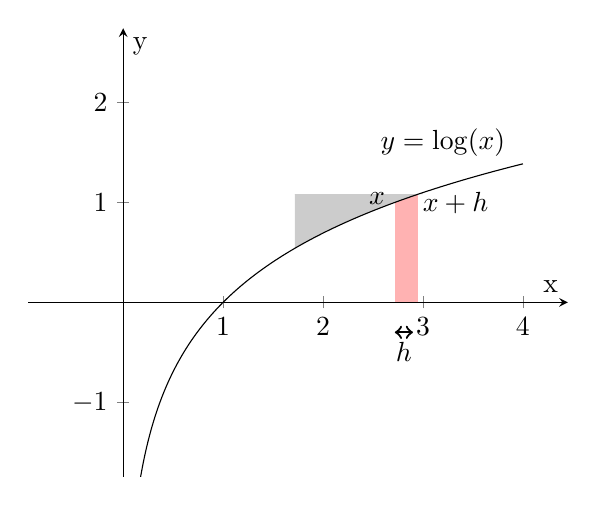
\begin{tikzpicture}
  \pgfdeclarelayer{pre main}
  \pgfsetlayers{pre main,main}
  \begin{axis}[
      axis lines = middle,
      axis equal,
      enlargelimits,
      domain  = 0:4,
      xlabel  = {x},
      ylabel  = {y},
      xmin    = -0.5,
      xmax    = 4,
      ymin    = -1,
      ymax    = 2,
      samples = 3000,
      mark    = none,
    ]
    \pgfonlayer{pre main}
    \fill[red!30] (e,0) rectangle (2.95,1.08180517035);
    \endpgfonlayer
    \addplot [name path=ln, thin]  {ln(x)};
    
    \addplot [name path=null, draw=none]  {1.08180517035};
    \addplot[color= mygray , opacity = 1] fill between[of=null and ln,
      soft clip={domain=e-1:3}];
    \node at (3.2,1.6) {$y = \log (x)$};
    \draw (e,1.2) node[ anchor =north east]{\ssmall$x$};
    \draw (2.9,1.2) node[ anchor = north west]{\ssmall$x+h$};
    \draw [black , thick , <-> ](e,-0.3) -- (2.9,-0.3) node[midway, below]{$h$};
    
  \end{axis}
\end{tikzpicture}\\
\end{tcolorbox}

\begin{tcolorbox}[width=\textwidth,colback={mygray},title={\begin{theorem} $\log x$ is differentiable and its derivative is $\frac{1}{x}$\end{theorem}},colbacktitle=myblue,coltitle=black]    
\underline{Proof:}\\ We will use the old but trustworthy trick of multiplying times one: $$h'(x)=\lim_{h\rightarrow0}\frac{f(g(x+h))-f(g(x))}{h}\frac{g(x+h)-g(x)}{g(x+h)-g(x)}$$
Let $k=g(x+h)-g(x)$, $u=g(x)$:
$$\lim_{h\rightarrow0}\frac{f(u+k)-f(u)}{k}\frac{g(x+h)-g(x)}{h}=f'(u)g'(x)$$
\end{tcolorbox}

\begin{tcolorbox}[width=\textwidth,colback={mygray},title={\begin{theorem} If $a,b>0$ then we have $\log(ab)=\log a+\log b$\end{theorem}},colbacktitle=myblue,coltitle=black]    
\underline{Proof:}\\  Let $f(x)=\log(ax)$ then $f'(x)+\frac{1}{x}$. As this is the derivative of $\log(x)$ we know that both functions must differ by a constant for all values. 
$$\log(ax)-\log(x)=k,\, k\in \mathbb{R}$$
Take $x=1$
$$\log(a)-log(1)=k=\log(a)$$
Then choose $x=b$
\end{tcolorbox}

\begin{tcolorbox}[width=\textwidth,colback={mygray},title={\begin{theorem} $\log(x)$ is strictly increasing $\forall x>0$. Its range is $(-\infty,\infty)$\end{theorem}},colbacktitle=myblue,coltitle=black]    
\underline{Proof:}\\
For the growth of the function we can use its derivative. 
\\
Pick any integer greater than one. By induction we can prove:$$\log(2^n)=n\log(2)$$. $\log(2)>0$ then we have that $\log(2^n)\longrightarrow \infty$ when $n\longrightarrow\infty$. That's half the range.
\\
for small values, $$0=\log(1)=\log(2^n 2^{-n})+\log(2^n)+\log(2^{-n})$$
$$\log(2^{-n})=-n\log(2^n)$$
So when $n$ goes to $\infty$, we have that $\log(2^{-n})\rightarrow -\infty$
\end{tcolorbox}
\begin{tcolorbox}[width=\textwidth,colback={mygray},title={\begin{definition}Exponential Function\end{definition}},colbacktitle=mygreen,coltitle=black] 
We define the exponential function as the inverse of $\log(x)$:
$$\exp:\; \R\longrightarrow (0,\infty)$$\\
We know it is well defined as the logarithmic function is bijective when its domain is $(0,\infty)$
\end{tcolorbox}
\begin{tcolorbox}[width=\textwidth,colback={mygray},title={\begin{theorem} $\forall x_1,x_2\in\R$ $$\exp(x_1+x_2)=\exp(x_1)\exp(x_2)$$
\end{theorem}},colbacktitle=myblue,coltitle=black] 
\underline{Proof:}\\ Set $a=\exp(x_1)$ and $b=\exp(x_2)$. Then by definition, $\log(a)=x_1$ and $\log(b)=x_2$. Evaluating, 
$$\exp(x_1+x_2)=\exp(\log(a)+\log(b))=\exp(\log(ab))=ab=\exp(x_1)\exp(x_2)$$
\end{tcolorbox}
\begin{tcolorbox}[width=\textwidth,colback={mygray},title={\begin{theorem}
$\exp(x)$ is differentiable $\forall x\in\R$ and its derivative is itself\end{theorem}},colbacktitle=myblue,coltitle=black]
\underline{Proof:}
\end{tcolorbox}
\section{Logarithmic differentiation}
Let $y=f(x)$, hard to differentiate using common techniques. Take $\log$ on both sides and define a new function. We then have $\log(y)=\log(f(x))=:g(x)$. Differentiating implicitly w.r.s. to $x$, $$\frac{y'}{y}=g'(x)$$
Then, solving for $y'$, $$y'=yg'(x)=f(x)g'(x)$$
\section{L'Hôpital's Rule}
First we will show the simplest case:
\begin{tcolorbox}[width=\textwidth,colback={mygray},title={\begin{theorem} $f,g$ differentiable on an open interval $I$ with $x_0\in I$. Suppose $f(x_0)=g(x_0)=0$ and that $g'(x_0)\neq 0$. Then $$\lim_{x\rightarrow x_0}\frac{f(x)}{g(x)}=\frac{f'(x_0)}{g'(x_0)}$$\end{theorem}},colbacktitle=myblue,coltitle=black]    
\underline{Proof:}\\  $$\lim_{x\rightarrow x_0}\frac{f(x)}{g(x)}=\lim_{x\rightarrow x_0}\frac{f(x)-f(x_0)}{g(x)-g(x_0)}=\lim_{x\rightarrow x_0}\displaystyle\frac{\displaystyle\frac{f(x)-f(x_0)}{x-x_0}}{\displaystyle\frac{g(x)-g(x_0)}{x-x_0}}= \frac{f'(x_0)}{g'(x_0)}  $$
By the properties of limits and the differentiability of $f$ and $g$.
\end{tcolorbox}


\newpage

\section{Brief Syllabus of Known Limits and Derivatives}

\newcommand{\limt}{\lim_{x \to 0}}
\newcommand{\lims}{\lim_{x \to x_0}}
\newcommand{\fr}{\frac{d}{dx}}

\section*{Limits}

\begin{enumerate}

    \item $$ \limt \frac{\sin x}{x}=1$$
    \item $$ \limt \frac{1-\cos x}{x}= 0$$
    \item $$ \limt \frac{1- \cos x}{x^2}=1$$
    \item $$ \lim_{x \to \pm \infty} \left( 1+\frac{1}{x} \right)^x=e$$
    \item $$ \limt \frac{\ln (1+x)}{x}=1$$
    \item $$ \limt \frac{e^x-1}{x}=1$$
    \item $$ \limt \frac{\log_a(1+x)}{x}= \log_a e$$
    \item $$ \limt \frac{a^x-1}{x}=\ln a$$
    \item $$ \limt \frac{(1+x)^k-1}{x}=k$$
    
\end{enumerate}


\section*{Derivatives}
\begin{enumerate}
    
    \item $$ \fr x^n=nx^{n-1}$$
    \item $$ \fr \sin x = \cos x$$
    \item $$ \fr \cos x = - \sin x$$
    \item $$ \fr e^x=e^x$$
    \item $$ \fr \log x = \frac{1}{x}$$
    \item $$ \fr \arctan x= \frac{1}{1+x^2}$$
    \item $$ \fr \arcsin x= \frac{1}{\sqrt{1-x^2}}$$
    \item $$ \fr \arccos x= -\frac{1}{\sqrt{1-x^2}}$$
    
    
\end{enumerate}


\chapter{Integration}

\section{Introduction}

\section{Riemann Integral}

\begin{definition}First, let us define the partition of an interval $[a,b]$ as a finite sequence of number such that:
$$a=x_0<x_1<x_2<\dots <x_n=b$$

Each $[a_i,x_{i+1}]$ is a \textbf{sub-interval} of the partition.
\subsubsection*{Partition of and Interval}
\end{definition}


\subsubsection*{Riemann Sums}
Now let $t_i\in [x_i,x_{x+1}]$. A Riemann sum is:

$$\sum_{i=0}^{n-1}f(t_i)(x_{i+1}-x_i)$$

Let the \textbf{Left Riemann sum} be defined as:

$$\sum_{i=0}^{n-1}f(x_i)(x_{i+1}-x_i)$$

Let the \textbf{Right Riemann sum} be defined as:

$$\sum_{i=0}^{n-1}f(x_{x+1})(x_{i+1}-x_i)$$

Let the \textbf{Middle Riemann sum} be defined as:

$$\sum_{i=0}^{n-1}f \left( \frac{x_{i+1}-x_i}{2} \right) (x_{i+1}-x_i)$$

\subsubsection*{Convergence}

For a one-dimensional Riemann sum over domain $[a,b]$, some functions* for \\ $n\to \infty$, if the integral exists, will have all the Riemann sums converge to the same value, which is defined as the \textbf{Riemann integral of the function $f$ over the interval $[a,b]$}.

$$\lim_{n\to \infty}\sum_{i=0}^{n-1}f(x_{i+1})(x_{i+1}-x_i)=\lim_{n\to \infty}\sum_{i=0}^{n-1}f(x_i)(x_{i+1}-x_i)=\int_a^bf(x)dx$$

*some functions are unfortunately non-Riemann integrable even if the integral exists. (Have a look at the Dirichlet function)

\subsection{Comparision Theorem}
\begin{theorem}
Let $f,g$ satisfy
\begin{enumerate}
    \item $\abs{f(x)} \leq g(x) $
    \item $\displaystyle\int_{a} ^{b} f , \displaystyle\int_{a} ^{b} g \exists$\\
\end{enumerate}
Then
\begin{enumerate}
    \item 
\end{enumerate}
\end{theorem}

\chapter{Integration}
\section{Classic integration}
We think of integrals as antiderivatives. Given $f(x)$, can I find $F(x)$ such that $F'(x)=f(x)$. We call $F(x)$ the indefinite integral of $f$, and it is not uniquely defined, as $F(x)+C$ is also an antiderivative of $f$ $\forall C\in\mathbb{R}$.
\paragraph{} We can also study integrals as the area under a curve, but both definition are consistent. This is what is fundamentally proven by the Fundamental Theorem of Calculus. $$\frac{dF}{dx}=f(x)=\lim_{h\rightarrow 0}\frac{F(x+h)-F(x)}{h}$$

\begin{theorem}
[Fundamental theorem of Calculus]Let $F'(x)dx=f(x)$. Then $$\int_a^bf(x)=F(a)-F(b)$$. \begin{proof} We have that $$F'(x_i)\approx \frac{F(x_i)-F(x_{x-1})}{h}$$
Then $$\int_a^bf(x)dx=\sum_{i=1}^n F'(x_i-1)h\approx\sum_{i=1}^nF(x_i)-F(x_{x-1})=F(b)-F(a)$$
\end{proof}
\end{theorem}
\begin{corollary} Integrating with functions as limits of integration:
$$\frac{d}{dx}\left(\int_a^{g(x)}f(t)dt\right)=f(g(x))g'(x)$$
\begin{proof}
This is a direct consequence of FTC
\end{proof}
\end{corollary}

\section{Improper integrals}
\begin{definition}
We have an improper integral when one of the bounds tends to $\infty$ or $f$ is unbounded at some point in $(a,b)$. We calculate improper integrals by taking the limit of proper integrals. 
\end{definition}
\begin{theorem}
[Comparison Theorem]
Let $f,g$ satisfy \begin{enumerate}[label=\textit{\roman*)}]
    \item $\vert f(x)\vert \leq g(x)$
    \item $\int_a^bf$ and $\int_a^bg$ exist for all $a,b\in\R$
\end{enumerate}
Then \begin{enumerate}
    \item If $\int_a^bg(x)dx<\infty\Longrightarrow\int_a^bf(x)dx<\infty$
    \item If $$\int_a^bf(x)dx>\infty\Longrightarrow\int_a^bg(x)dx>\infty$$
    \end{enumerate}
    \begin{proof} The proof is intuitive, as the inequalities in functions are reflected also in the area under their graph.
    \end{proof}
\end{theorem}
\section{Mean Value theorem for integrals}

\section{Applications of integrals}
\subsection{Length of curves}
$$L=\int_{t_0}^{t_1}\left[\left(\frac{dx}{dt}\right)^2+\left(\frac{dy}{dt}\right)^2\right]^{1/2}dt$$
\subsection{Volumes}
$$V=\int_a^bA(x)dx$$
\paragraph{Volumes of revolution}
Around the x-axis
$$V=\pi \int ^{b}_{a}\left( f\left( x\right) \right) ^{2}dx$$
Around the y-axis
$$V=2\pi \int ^{b}_{a}xf\left( x\right) dx$$
\subsection{Surface areas}
$$A=2\pi \int ^{b}_{a}f\left( x\right) \sqrt {1+\left( f'\left( x\right) \right) ^{2}}dx$$

\subsection{Center of mass}
In 1D we can calculate the center of mass of a finite number of masses by considering their individual torque contributions, and finding the point where their sum is zero. Therefore $$\sum ^{n}_{i=1}m_{i}\left( \overline {x}-x_{i}\right) =0\Rightarrow \overline {x}\sum ^{n}_{i=i}m_{i}=\sum m_{i}x_{i}\Leftrightarrow \overline {x}=\dfrac {\sum ^{n}_{i=1}x_{i}m_{i}}{M}$$
For 2D we have the same procedure but in two variables. 


For continuous mass distributions we need to partition the area under study.
$$\Delta M_{y_{ij}}=\left( \overline {x}-x_{i}\right) \rho \left( x_{i},y_{j}\right) \Delta x\Delta y$$
$$M_{y}=\int \int _{R}\left( \overline {x}-x\right) \rho \left( x,y\right) dxdy=0$$
$$\overline {x}=\dfrac {\int \int_R x\rho \left( x,y\right) dxdy}{M}$$
When we can bound the area between the x-axis and $y=f(x)$ we have 



\end{document}
%Note to self - start spending less time on Overleaf